\chapter{Datasets} \label{datasets}
Due to the varying definition of bias, different datasets aim to capture different angles of bias. In this section, I present a collection of all datasets related to biased writing and subjectivity detection available.

Because there are not many media bias datasets of sufficient quality, I included other relevant datasets which are at least on some level related to the media bias and later leveraged their bias information to augment smaller ground truth datasets. I will discuss this approach in experiment section \ref{experiments}.

As discussed in \ref{methodology} this work only focuses on sentence level classification, thus datasets that focus only on article level bias information were excluded.



\subsection[SUBJ]{SUBJ \cite{Pang+Lee:04a}}
The Subjectivity dataset (SUBJ) \cite{Pang+Lee:04a} consists of 10000 sentences gathered from movie review sites. Sentences are labeled as subjective and objective with 1:1 ratio. 

The data were collected in an automatic way, thus the labels can be assumed to be noisy. The authors made an assumption that all reviews from Rottentomatoes\footnote{https://www.rottentomatoes.com/} are subjective and all plot summaries from IMBD\footnote{ www.imdb.com} are objective. Then 5k of sentences were sampled randomly for each class.




\subsection{MPQA}
\textbf{M}ulti-\textbf{P}erspective \textbf{Q}uestion \textbf{A}nswering (MPQA) Opinion corpus is another dataset that can be used for subjectivity detection. For the purpose of our task, I used the MPQA Opinion corpus version 2.0, which consists of 692 articles from 187 different news sources summing up to 15,802 sentences. All articles are from June 2001 to May 2002.

The corpus offers a rich annotation scheme \cite{wiebe2005annotating} that focuses on sentiment and subjectivity annotations.
\newpage
To extract the bias information, I focused on two types of annotations:
\begin{itemize}
    \item Direct subjective
    \item Expressive subjective
\end{itemize}
Which were present in any form of subjectivity was suspected. Each annotation consists of indices of span in the text and properties. For each sentence in corpus I extracted labels as follows:

If there was at least one annotation \textbf{direct\_subjective} or \textbf{expressive\_subjectivity} with span inside the sentence and the intensity tag was not $low$, the sentence was labelled as subjective/biased. All other sentences were extracted as objective/unbiased.

This approach yielded $9,484$ subjective sentences and 6318 objective sentences.




\subsection{BASIL}
BASIL dataset \cite{fan2019plain} comprise 300 articles with 1,727 sentence level bias annotations. The authors of the dataset distinguish between \textbf{lexical} and \textbf{informational} bias. Here, lexical bias is defined as a form of bias which does not depend on the context and usually introduces polarized words.

The annotations were performed by two experts and further resolution discussions later led to 0.56 and 0.7 \Gls{iaa} score for lexical and informational bias, respectively.

Even though BASIL brings the sufficient annotation quality, most of the labelling resulted in informational bias annotations, leaving only 478 sentences with lexical bias information. Informational bias requires a different approach to detection \cite{van2020context} and usually depends on context dramatically. Therefore,in terms of media bias detection, I extracted all sentences with 'informational' label as a neutral class.




\subsection{Ukraine Crisis Dataset}
This dataset \cite{farber2020multidimensional} offers 2057 sentences with annotation of media bias. All sentences are related to one topic - Ukraine-Russian crisis and data were gathered from 90 news sources.

The authors introduce rich annotations for each sentence. Each one of them looking at the bias from a different perspective, so called \textit{bias dimensions}.
\begin{enumerate}
    \item Hidden Assumptions and Premises
    \item Subjectivity
    \item Framing
\end{enumerate}
In addition, the \textit{overall bias} annotation is presented. Together, the data involve 44 547 fine-grained annotations. For media bias detection, only overall bias annotations were used.
Even though this is one of the highest quality dataset regarding media bias, specifically, it also suffers from low Krippendorff’s alpha score (~ -0.05). Therefore, its usability is limited. 




\subsection{NFNJ}
The NFNJ\footnote{\cite{farber2020multidimensional} refer to this dataset as NFNJ, however in the original paper the name is not presented.} dataset provides 966 sentences from 46 articles with annotations on a fine-grained level. Despite the relatively small size of the dataset, the \Gls{iaa} measures Fleiss Kappa scores of zero on average.

Authors share the dataset for research purposes, however, the public version differs from the one described in the original paper. In creating the final dataset, I made a few assumptions:

In the raw data, contributions from multiple annotators on each sentence are provided. Therefore, I extracted the labels as a simple arithmetical mean of the labels. Furthermore, the original labels stand for 
\begin{itemize}
    \item 1: 'neutral'
    \item 2: 'slightly biased but acceptable'
    \item 3: 'biased'
    \item 4: 'very biased'
\end{itemize}
To obtain the final truth labels in a neutral/biased format, I simply assumed sentences with score $\leq$ 2 as neutral and $>$ 2 as biased.




\subsection{BABE}
A key media bias dataset from \Gls{mbg}, which is to the best of my knowledge and according to the authors, the highest quality media bias dataset to this day. It builds on top of MBIC \cite{Spinde2021MBIC} which is a smaller crowdsourced dataset.

BABE contains 3700 sentences. 1700 sentences are from MBIC, which were extracted from 1000 news articles, and in addition extended by 2000 more sentences, altogether covering 12 topics.

BABE has been annotated by 8 experts resulting in \gls{iaa} Krippendorfs $\alpha = 0.46$, which exceeds other media bias datasets by a large margin.It also provides detailed information about the annotator background, making it a \textbf{reliable} source of bias information. The scheme of collection of sentences and labelling can be seen in \ref{fig:babe-data}

\begin{figure}
  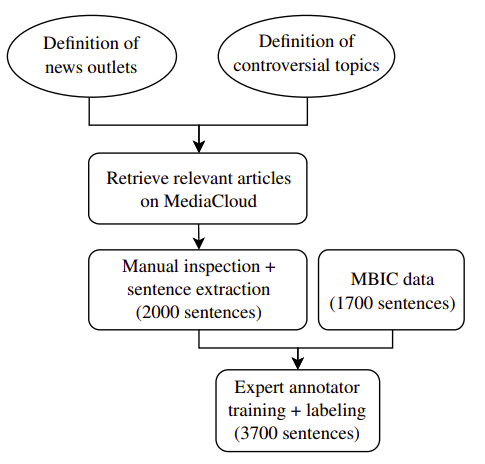
\includegraphics[width=\linewidth]{my_modules/multimedia/babe.png}
  \caption{Data collection and annotation pipeline}
  \label{fig:babe-data}
  \cite{Spinde2021f}
\end{figure}

\section{Wikipedia NPOV datasets}\label{wiki-npov}
Due to annotation costs and the overall lack of large-scale datasets in media bias settings, many researches \cite{pryzant2020automatically,recasens2013linguistic,hube2019neural} used Wikipedia's \Gls{npov} policy\footnote{\url{https://en.wikipedia.org/wiki/Wikipedia:Neutral_point_of_view}}. to construct large-scale datasets automatically. 

Wikipedia's NPOV policy is a set of rules which aim to preserve neutrality in Wikipedia texts. Some examples of NPOV principles are:
\begin{itemize}
    \item Avoid stating opinions as facts.
    \item Avoid stating facts as opinions.
    \item Prefer nonjudgmental language.
\end{itemize}
When neutrality is contested, Wikipedia article can be moved to NPOV dispute by tagging it with \{\{NPOV\}\} or \{\{POV\}\} template. Debate on specific details of neutrality violations is then initialized among editors and eventually resolved, leading to removal of the tag.

This editorial information can be used to extract parts of the text that violate NPOV and their unbiased counterparts. However, it has been shown \cite{hube2019neural,zhong-etal-2021-wikibias-detecting} that such automatic extraction can suffer from noisy labelling. In some cases \cite{hube2019neural} up to 60\% of data positive points were actually neutral.

Even though these datasets introduce a large amount of samples that are highly related to media bias, they are all sampled from Wikipedia's environment, which can be very different from the news environment. 




\subsection{Wiki Neutrality Corpus}\label{wiki}
\Gls{wnc} \cite{pryzant2020automatically} is a parallel corpus of 180k pairs of biased and unbiased sentences. For the collection of the data, \ref{wiki-npov} approach was adopted. The authors crawled revisions of wikipedia from time span 2014 - 2019. Each revision has been processed to check if it contains any variation of \textit{POV} related text in it. This aproach yielded 180k pairs such that sentence before edit is considered biased and modified/added sentence after edit is considered to be neutral/unbiased.
    
In addition to WNC, 385k of sentences which have not been changed during the NPOV dispute were extracted as neutral and for word-level classification purposes, a subset of WNC corpus, where only one word is changed in the biased-unbiased pair, were added.




\subsection{CW-HARD}
Hube et. al \cite{hube2019neural} constructed dataset based on NPOV, where only revisions with one sentence diff were filtered. However, because of the potentially noisy outcome, 5000 sentences were sampled and annotated using crouwdsourcing. Yet, the Krippendorffs Alpha agreement score measured only $\alpha = 0.124$ which is generally considered low. 

After filtering out sentences which annotators labeled with "I dont know" option, the final dataset consists of 1843 statements labeled as biased and 3109 labeled as neutral, a total of 4953 sentences.

\begin{table}
\begin{ctucolortab}
\begin{tabular}{c|c|c|c}
 \textbf{Dataset} & \textbf{Size} & \textbf{Annotation} & \textbf{Agreement}\\
 \hline
 \textbf{SUBJ} & 10.000 & automatic & -\\ 
 \hline
 \textbf{MPQA} & 15.802 & annotators & high \\
 \hline
 \textbf{BASIL} &  1.727 & annotators & medium \\ 
 \hline
 \textbf{Ukraine Crisis Dataset} & 2.057 & crowdsourcing & low \\ 
 \hline
 \textbf{NFNJ} & 888 & crowdsourcing & low \\
 \hline
 \textbf{BABE} & 3700 & annotators & medium \\
 \hline 
 \textbf{WNC} & 362.990 & automatic & - \\
 \hline
 \textbf{CW-hard} & 4953 & crowdsourcing & low \\
 \hline 
 \textbf{WikiBias} & 8198 & annotators & high \\
 \hline
\end{tabular}
\end{ctucolortab}
\caption{Comparison of all bias related datasets collected}
\label{table:1}
\end{table}


\subsection{WikiBias}
This is the latest dataset based on Wikipedia. The authors closely follow the approach of WNC \cite{pryzant2020automatically} and extract another parallel wiki corpus of 214k sentences.
To achieve a higher quality corpus, 4099 sentence pairs were randomly sampled and labeled by trained annotators. As a result, introduced WikiBias-Manual dataset consists of 3,400 biased and 4,798 neutral sentences annotated with high \gls{iaa} Cohen's $\kappa = 0.734$




\section{Unused datasets}
 Some datasets focus on a slightly different task, yet still carry potentially useful information. Such data can be useful in a Multi-Task setting \ref{mtl}. To name a few, mainly Ideology detection focused, data:
\begin{itemize}
\item \textbf{NewsB} - 
Consists of labels capturing authors political ideology (liberal, conservative)
\item \textbf{IBC} - Also focuses on ideology detection, however,it is not publicly available and I was not able to get the dataset from the authors
\end{itemize}


\section{Datasets summary}
In the previous section, I introduced all resources that are potentially useful for media bias analysis and are publicly available. The overview of all datasets and its properties can be seen in figure \ref{table:1}.
